\documentclass{standalone}

\usepackage{tikz}
\usetikzlibrary{angles,quotes}
\usepackage{amsmath,amssymb,amsfonts,xcolor}

\usepackage{pgfplots}
\definecolor{darkgreen}{rgb}{0.0, 0.42, 0.24}
\definecolor{amethyst}{rgb}{0.6, 0.4, 0.8}

\pgfplotsset{compat=newest}
\pgfplotsset{every axis/.append style={
                     tick label style={font=\footnotesize},
                 }}

\begin{document}
      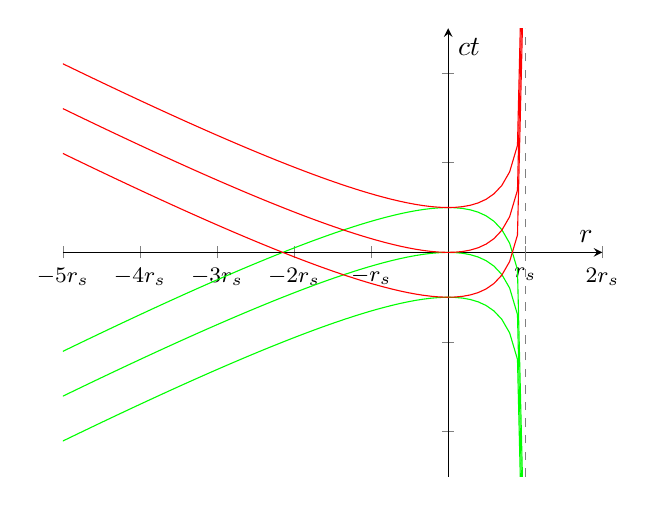
\begin{tikzpicture}
        \begin{axis}[xmin=-5,xmax=2,ymin=-5,ymax=5,
        xtick={-5,-4,-3,-2,-1,0,1,2},
        xticklabels={$-5r_{s}$,$-4r_{s}$,$-3r_{s}$,$-2r_{s}$,$-r_{s}$,$0$,$r_{s}$,$2r_{s}$},
        yticklabels=false,
        axis lines = middle,
        xlabel=$r$,
        ylabel=$ct$,
        domain=-5:1]
            \addplot[color=green,samples=60]{x+ln(-x+1)};
            \addplot[color=green,samples=60]{x+ln(-x+1)+1};
            \addplot[color=green,samples=60]{x+ln(-x+1)-1};
            \addplot[color=red,samples=60]{-x-ln(-x+1)};
            \addplot[color=red,samples=60]{-x-ln(-x+1)+1};
            \addplot[color=red,samples=60]{-x-ln(-x+1)-1};
           \addplot[color=gray,dashed,samples=30] coordinates {(1,-5)(1,5)};
        \end{axis}
    \end{tikzpicture}
\end{document}